\chapter{Transport domain analysis}

In this chapter, we will analyze two variants of the Transport domain: sequential and temporal. To do this, we will describe a system we developed for the analysis
and development of planners for Transport, describe and analyze the datasets
used for devising experiments, and discuss the properties of Transport
that will help us in developing better quality planners.

\section{TransportEditor -- A Transportation Planning System}\label{transport-editor}

To enable effective transportation planning,
we have developed \textit{TransportEditor}, a system for creating and visualizing transportation problems and plans.
Specifically, TransportEditor aims to be a problem editor and plan visualizer for the Transport domain (and its variants). It is an intuitive and cross-platform graphical desktop application (Figure~\ref{fig:transporteditor-screenshot})
written in Java.

It allows the user to create a planning session, where they
select a Transport domain variant, load a problem instance from PDDL (Section~\ref{pddl}) or create a new one from scratch.
The road network of the problem is automatically laid out and visualized for the user as a graph with locations as nodes and roads as edges.
Users can then tweak the layout, make changes to vehicle and package properties
and export the problem or domain back into PDDL.

They can also select an external planner
referencing its executable file, or select one of the built-in planners and try to solve
the loaded problem using the selected planner. Internal and external plan validators, like VAL \citep{Howey2003}, can also be selected to verify plans are correct.
Once plans are loaded and verified, it will let the user see a list of actions
in the plan, or plot a Gantt chart (useful for observing concurrent actions in temporal domain variants).

The best feature of TransportEditor is the option of tracing plans. We can select
any action, specify an exact time point or just step through the actions in order and
the road network on the left will display the current state of the problem, as if
all actions before the current point were applied to the start state.
It is possible to do all of this, and more, without ever leaving the TransportEditor user interface.

TransportEditor will help researchers working on this domain fine-tune their planners; they can visualize the various corner cases their planner fails to handle, step through the generated plan and find the points where their approach fails.
A secondary motivation is to be able to test approaches for creating plans for the domain.
For screenshots of typical TransportEditor usage, see the attached \nameref{transport-editor-screenshots}.

\begin{figure}[t]
\begin{center}
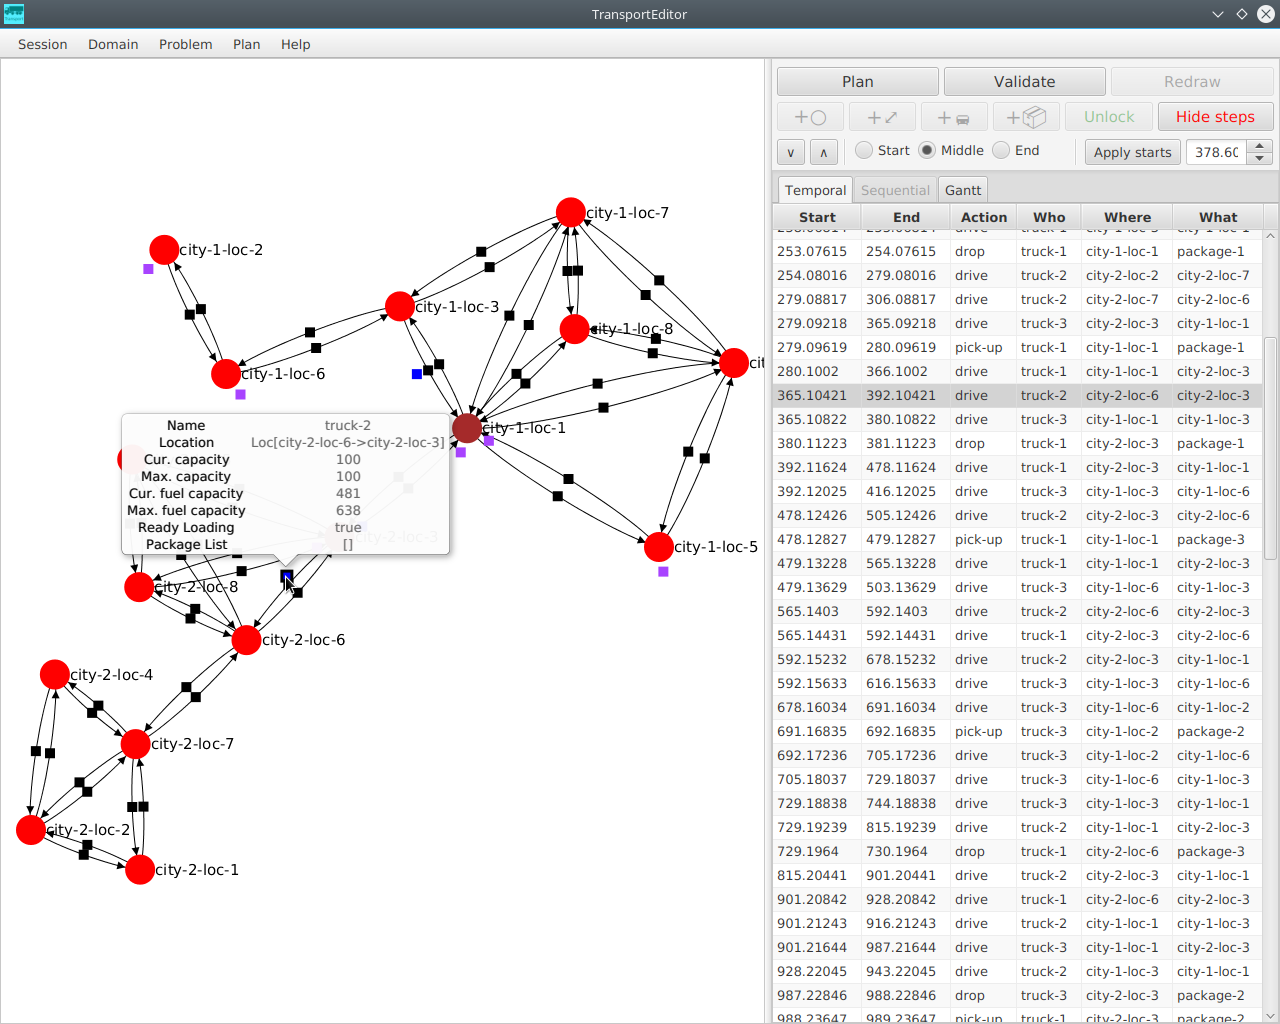
\includegraphics[width=0.9\textwidth]{../img/transporteditor_temporal}
\end{center}
\caption[Screenshot of a user tracing actions of a plan for a small temporal problem in TransportEditor.]{Screenshot of a user tracing actions of a plan for a small temporal problem in TransportEditor. The bubble in the middle shows details
of a truck currently driving along a road between \texttt{city-2-loc-6} and \texttt{city-2-loc-3}. The \texttt{city-1-loc-1} location is plotted in a darker shade of red, which signifies that a petrol station is present at the location.}
\label{fig:transporteditor-screenshot}
\end{figure}

The basic user workflow of TransportEditor consists of the following steps:
\begin{itemize}
\item Selecting which formulation of the Transport domain they want to work with or create their own variant;
\item Loading the PDDL or creating their own problem of the given domain. TransportEditor then visualizes the given graph as good as it can;
\item Iterating among the following options:
\begin{itemize}
\item Loading a planner executable and letting TransportEditor run the planner on the loaded problem instance for a given time (the user can cancel anytime),
then loading the resulting plan;
\item Possibly loading a pre-generated plan;
\item Stepping through the individual plan actions and letting TransportEditor visualize them.
The user can step forward and backward in the plan and inspect each action result in great detail;
\item Editing the graph: adding/removing/editing the location or properties of vehicles, packages, roads, locations and possibly petrol stations;
\item Saving the currently generated plan;
\item Saving the problem;
\item Saving the domain (exporting to a PDDL file).
\end{itemize}
\item Saving and closing the currently loaded problem. Exit the application or go back to the first step.
\end{itemize}

TransportEditor is a part of this thesis and you can find it on the attachment CD (see the attached \nameref{cd-contents} for more information). Both the \nameref{transporteditor-user-manual},
the \nameref{transporteditor-developer-manual}, and the \nameref{transporteditor-developer-javadoc} are attached to this thesis in a digital format, offering guidance when
using the program and providing an in-depth description.
















\section{Properties of Transport domains}

In this section, we will delve more deeply into the Transport domain and try to analyze its properties.
We will describe the problem instances that have been used in the IPC and discuss insights useful for devising heuristics or for other approaches to creating plans for these problems.

\subsection{Does domain knowledge make Transport easy to solve?}

When domain-independent planners solve a sequential Transport problem,
they face a harder task than our planners that have domain knowledge ahead of time.
Deciding whether a plan of a given length exists is, in the case of Transport,
an NEXPTIME-complete task \citep[Section~3.4]{Ghallab2004}.
That does not mean domain knowledge makes Transport easy. We will now show
that even the sequential variant of Transport is NP-hard.

\begin{thm}
The problem of finding an optimal plan for an undirected connected graph in the sequential
Transport domain is NP-hard. \TODO{Formulate better and revise proof}
\end{thm}
\begin{proof}
It is not evident if the problem is in NP: if we get a plan, there is no straightforward
way of verifying whether it is optimal.

We will now show that we can reduce an NP-complete problem to our problem in polynomial time,
hence proving that all NP-complete problems are reducible to our problem,
and therefore, our problem is NP-hard.

As proven by \citet{Karp1972}, the problem of existence of a Hamilton circuit (HC) in a (directed or undirected) graph is NP-complete. We will show that we are able to transform the HC problem into a sequential Transport problem.

Given an undirected graph $G$, the solution to HC is a cycle through all the nodes of $G$,
without visiting any single node twice.
We can use the same graph to model a Transport problem instance.
The problem will contain only one vehicle of capacity $n-1$,
where $n = |G|$, the number of nodes in the graph.

We will co-locate $n-1$ packages with the vehicle at any predetermined graph vertex $l \in G$.
One package $p'$ will be located elsewhere, at $l' \in G,\, l \neq l'$.
Each package positioned at $l$ will have a different target than the other packages at $l$
and none of the targets will be $l$. The package at $l'$ will have the original node $l$
as its target. We will set all road lengths to $1$. 

An optimal plan for the designed translation has a total cost of at least $3n$.
Any plan for this problem has to have at least $n$ \verb+drive+ actions, because
there is a package to be delivered to every node, and the graph has $n$ nodes.
Because it has to move $n$ packages, at least $n$ \verb+pick-up+ and $n$ \verb+drop+
actions are needed. The costs of all actions are 1.
We conjecture that an HC exists if and only if an optimal and valid plan visits each vertex only once.

First, we prove the forward implication. Assume an HC exists and the optimal plan visits at least one node twice. We can now construct a plan with a lower total cost than the optimal plan: first, pick up all the $n-1$ co-located packages, then drive along the HC. At each
visited node, drop the package that has this node as its destination. If we are at $l'$,
pick up the package $p'$. The plan is trivially valid, as it delivers all packages
and the vehicle never over-reaches its capacity. Also, its total cost is $3n$
(the length of the HC is $n$, which implies $n$ drive actions) and for every of the $n$ packages, we do exactly one \verb+pick-up+ and exactly one \verb+drop+. Hence, the plan
is optimal and visits each vertex only once.

Now, assume an HC does not exist. If the found optimal plan only visits each node once,
we can look at the source locations of all \verb+drive+ actions and the target
location of the last \verb+drive+ action. They constitute a path through the graph on which a node never repeats and the path starts and finishes at the same node.
Hence, we have constructed a HC.
\end{proof}


\subsection{Datasets \& problem instances}

For evaluation and comparison with other planners, we have acquired several problem datasets from previous runs of the IPC.
Table~\ref{tab:ipc-datasets} provides an overview of the individual datasets, their associated IPC competition, the track at the competition and the domain variant the problems are modeled in.

\begin{table}[tb]
\begin{tabular}{c||ccc}
\textbf{Dataset} & \textbf{Competition} & \textbf{IPC Track} & \textbf{Formulation} \\ 
\midrule
\midrule
netben-opt-6 & IPC-6 & \href{http://icaps-conference.org/ipc2008/deterministic/NetBenefitOptimization.html}{Net-benefit: optimal} & Numeric \\ 
seq-opt-6 & IPC-6 & \href{http://icaps-conference.org/ipc2008/deterministic/SequentialOptimization.html}{Sequential: optimal} & STRIPS \\ 
seq-sat-6 & IPC-6 & \href{http://icaps-conference.org/ipc2008/deterministic/SequentialSatisficing.html}{Sequential: satisficing} & STRIPS \\ 
tempo-sat-6 & IPC-6 & \href{http://icaps-conference.org/ipc2008/deterministic/TemporalSatisficing.html}{Temporal: satisficing} & Temporal \\ 
\midrule
seq-agl-8 & IPC-8 & \href{https://helios.hud.ac.uk/scommv/IPC-14/seqagi.html}{Sequential: agile} & STRIPS \\ 
seq-mco-8 & IPC-8 & \href{https://helios.hud.ac.uk/scommv/IPC-14/seqmulti.html}{Sequential: multi-core} & STRIPS \\ 
seq-opt-8 & IPC-8 & \href{https://helios.hud.ac.uk/scommv/IPC-14/seqopt.html}{Sequential: optimal} & STRIPS \\ 
seq-sat-8 & IPC-8 & \href{https://helios.hud.ac.uk/scommv/IPC-14/seqsat.html}{Sequential: satisficing} & STRIPS \\ 
\end{tabular}
\caption{Transport datasets from the 2008 and 2014 IPCs.}
\label{tab:ipc-datasets}
\end{table}

Short descriptions of the various tracks and subtracks can be found in the rule pages of IPC-6\footnote{\url{http://icaps-conference.org/ipc2008/deterministic/CompetitionRules.html}}
and the rule pages of IPC-8\footnote{\url{https://helios.hud.ac.uk/scommv/IPC-14/rules.html}}.
Unfortunately, we weren't able to acquire the datasets for IPC-7 (2011), as the Subversion repository\footnote{\url{http://www.plg.inf.uc3m.es/ipc2011-deterministic/Domains.html}} that promises to contain them is unavailable.

We have decided to split our further research based on the tracks at IPC: we will focus on constructing
Transport-specific planners for the seq-sat-6, seq-sat-8, and tempo-sat-6 datasets,
corresponding to the sequential and temporal variants of Transport.

In addition to the domain definition, we need to take a look at the individual problems to fully utilize our knowledge advantage.
Both the seq-sat-6 and tempo-sat-6 contain 30 problems, while seq-sat-8 only contains 20. Table~\ref{tab:dataset-dimensions} shows the
dimensions of each problem instance for each mentioned dataset.

While the planners (including our domain-specific ones) do not know this,
each of the datasets was constructed with a scenario in mind. Locations in problems are not just
placed randomly, but usually belong to cities. Inside a city, the road network
tends to be dense and road lengths small, while roads connecting cities
are rare and usually significantly longer.


\begin{figure}[tb]
\begin{center}
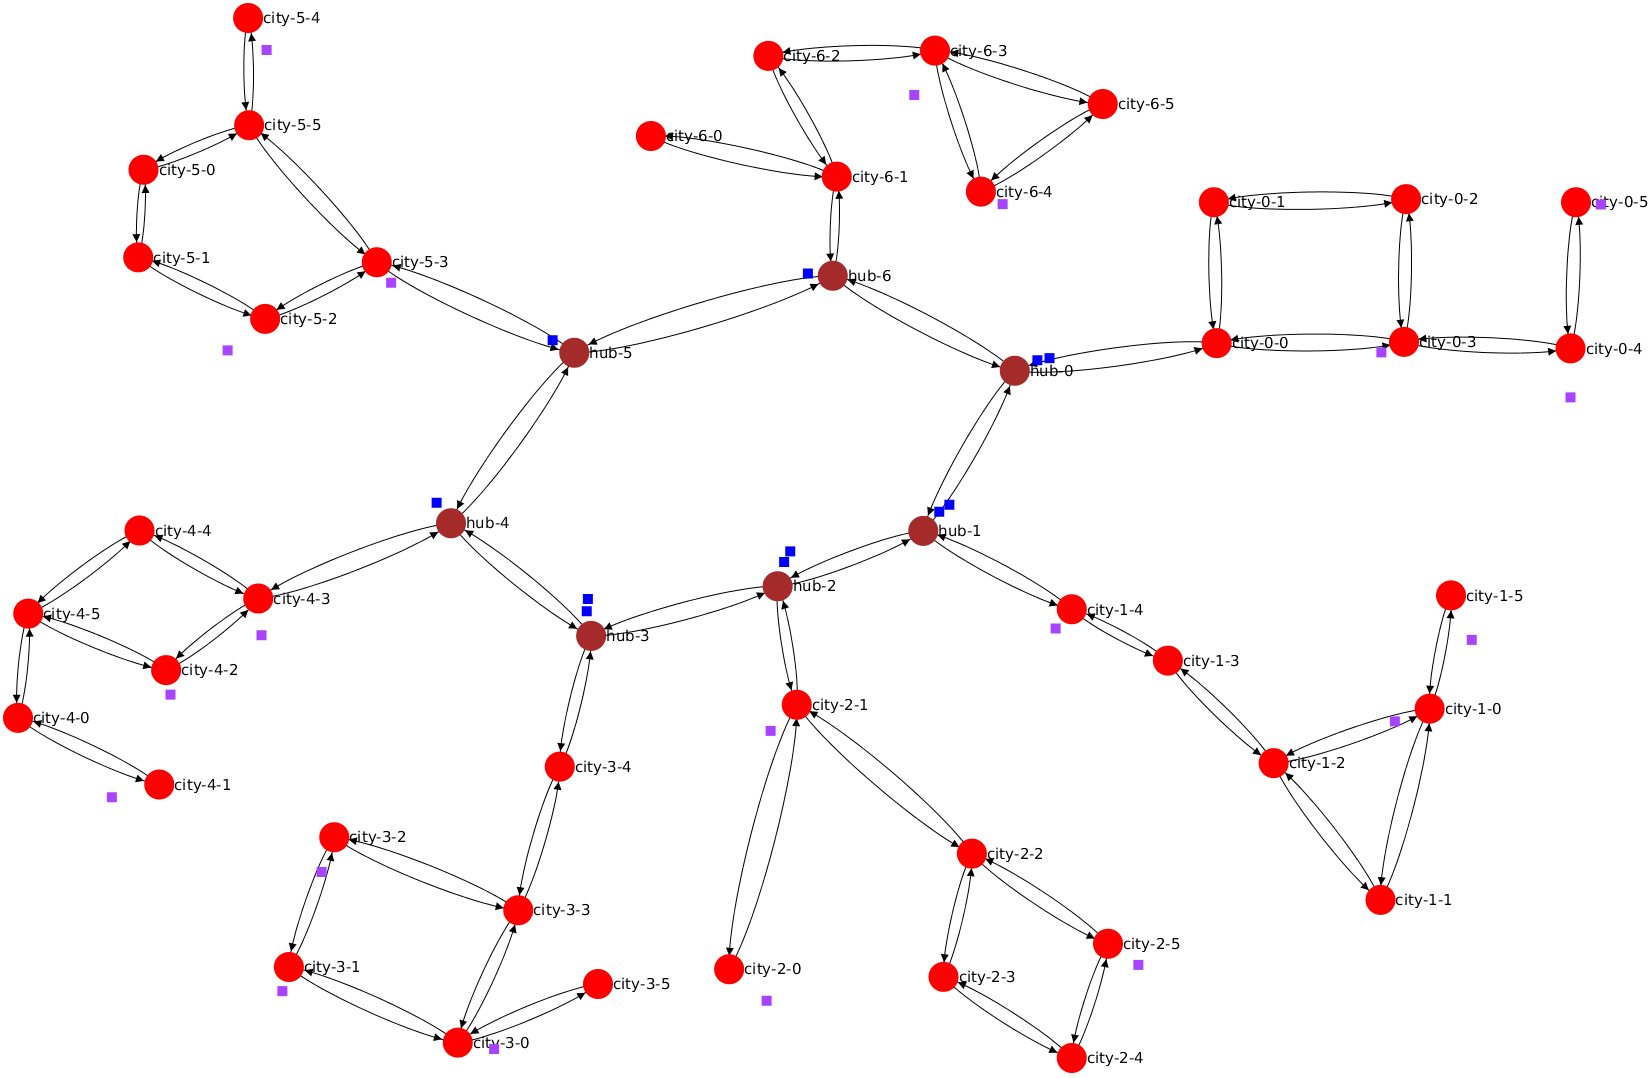
\includegraphics[width=1.0\textwidth]{../img/ipc08_tempo-sat_p30_land}
\end{center}
\caption[Visualization of the \texttt{p30} problem of temporal Transport from IPC 2008.]{Road graph visualization of the \texttt{p30} problem of the tempo-sat track of IPC 2008. Red dots represent locations (graph nodes), roads (graph edges) are represented by black arrows, vehicles are plotted as blue squares, and packages as purple squares. Darker red dots represent locations with petrol stations. In this specific problems, the circle of nodes in the center represents a series of truck hubs and each of the attached subgraphs are individual cities.}
\label{fig:ipc08_tempo-sat_p30}
\end{figure}

\begin{table}[p]
\footnotesize
\centering
\begin{subtable}[t]{0.42\textwidth}
\csvreader[tabular=r||rrrr,
    table head=\textbf{\#} & \rot{\textbf{Vehicles}} & \rot{\textbf{Packages}} & \rot{\textbf{Locations}} & \rot{\textbf{Roads}}\\\midrule\midrule,
    late after line=\mbox{}]
%    table foot=\\\bottomrule]%
{../data/seq-sat-6.csv}{Problem=\problem,Vehicles=\vehicles,Packages=\packages,Locations=\locations,Roads=\roads}%
{\problem & \vehicles & \packages & \locations & \roads}%
\caption{Problem dimensions of the seq-sat-6 dataset.}
\label{tab:seq-sat-6-dims}
\end{subtable}
\quad
\begin{subtable}[t]{0.54\textwidth}
\csvreader[tabular=r||rrrrr,
    table head=\textbf{\#} & \rot{\textbf{Vehicles}} & \rot{\textbf{Packages}} & \rot{\textbf{Locations}} & \rot{\textbf{Roads}} & \rot{\textbf{Petrol}}\\\midrule\midrule,
    late after line=\mbox{}]
%    table foot=\\\bottomrule]%
{../data/tempo-sat-6.csv}{Problem=\problem,Vehicles=\vehicles,Packages=\packages,Locations=\locations,Roads=\roads,PetrolStations=\petrol}%
{\problem & \vehicles & \packages & \locations & \roads & \petrol}%
\caption{Problem dimensions of the tempo-sat-6 dataset.}
\label{tab:tempo-sat-6-dims}
\end{subtable}

\begin{subtable}[t]{1\textwidth}
\vspace{0.5cm}
\begin{subtable}[t]{0.42\textwidth}
\csvreader[tabular=r||rrrr,
    table head=\textbf{\#} & \rot{\textbf{Vehicles}} & \rot{\textbf{Packages}} & \rot{\textbf{Locations}} & \rot{\textbf{Roads}}\\\midrule\midrule,
    late after line=\mbox{}]
%    table foot=\\\bottomrule]%
{../data/seq-sat-8.csv}{Problem=\problem,Vehicles=\vehicles,Packages=\packages,Locations=\locations,Roads=\roads}%
{\problem & \vehicles & \packages & \locations & \roads}%
\end{subtable}
\quad
\begin{subtable}[t]{0.54\textwidth}
\csvreader[tabular=r||rrrr,
    table head=\textbf{\#} & \rot{\textbf{Vehicles}} & \rot{\textbf{Packages}} & \rot{\textbf{Locations}} & \rot{\textbf{Roads}}\\\midrule\midrule,
    late after line=\mbox{}]
%    table foot=\\\bottomrule]%
{../data/seq-sat-8_2.csv}{Problem=\problem,Vehicles=\vehicles,Packages=\packages,Locations=\locations,Roads=\roads}%
{\problem & \vehicles & \packages & \locations & \roads}%
\end{subtable}
\caption{Problem dimensions of the seq-sat-8 dataset.}
\label{tab:seq-sat-8-dims}
\end{subtable}
\caption[Problem dimensions of selected Transport IPC datasets.]{Problem dimensions of selected Transport IPC datasets. Bolded problem instance numbers correspond to Figure~\ref{fig:ipc08_seq-sat_p13} and Figure~\ref{fig:ipc08_tempo-sat_p30} respectively.}
\label{tab:dataset-dimensions}
\end{table}


All sequential problem instances in seq-sat-6 and seq-sat-8 have symmetric roads and road lengths and can, therefore,
be simplified by assuming the use of an undirected graph.
In no sequential problem do vehicles need to finish at a specific target location.

The temporal problems in tempo-sat-6 do not have the same property;
the problems 1--20 have symmetric roads and lengths, but
the 21--30 problems only have symmetric roads, not lengths in general.
The same applies to fuel demands of roads and as a bonus,
these problems have vehicle target locations, which means that not only packages,
but also
vehicles will need to be positioned at specific locations
after package delivery finishes. We can interpret this goal
in a similar way as in a VRP, where a vehicle target location is thought to be
a truck depot or hub. A visualization of such a problem can be seen in Figure~\ref{fig:ipc08_tempo-sat_p30}.

\TODO{describe state space size + add to table}

We can see that problems vary not only in size but also in what features they include
and what assumptions they make.
A summary of the acquired insights is available in Table~\ref{tab:problem-properties}.

\begin{table}
\centering
\begin{tabular}{cc||ccccc}
\textbf{Dataset} & \textbf{Problems} & \rot{\textbf{\# of cities}} & \rot{\textbf{Symmetric road lengths}} & \rot{\textbf{Symmetric fuel demands}} & \rot{\textbf{Vehicle target locations}} & \rot{\textbf{State space size}}\\
\midrule
\midrule
\multirow{3}{*}{seq-sat-6} & 01--10 & 1 & \multirow{3}{*}{Yes} & \multirow{3}{*}{N/A} & \multirow{3}{*}{No} & • \\ 
& 11--20 & 2 &  &  &  & • \\ 
& 21--30 & 3 &  &  &  & • \\\midrule%
%
\multirow{6}{*}{seq-sat-8} & 01--03 & 1 & \multirow{6}{*}{Yes} & \multirow{6}{*}{N/A} & \multirow{6}{*}{No} & • \\ 
& 04--06 & 2 &  &  &  & • \\ 
& 07--10 & 3 &  &  &  & • \\ 
& 11--13 & 1 &  &  &  & • \\ 
& 14--16 & 2 &  &  &  & • \\ 
& 17--20 & 3 &  &  &  & • \\\midrule%
%
\multirow{7}{*}{tempo-sat-6} & 01--10 & 1 & Yes & Yes & No & • \\ 
& 11--20 & 2 & Yes & Yes & No & • \\\cmidrule{2-7}
& 21--22 & 3 & \multirow{5}{*}{No} & \multirow{5}{*}{No} & \multirow{5}{*}{Yes} & • \\ 
& 23--24 & 4 &  &  &  & • \\ 
& 25--26 & 5 &  &  &  & • \\ 
& 27--28 & 6 &  &  &  & • \\ 
& 29--30 & 7 &  &  &  & •
\end{tabular} 
\caption{Summary of problem instance properties in IPC Transport datasets.}
\label{tab:problem-properties}
\end{table}

\subsection{Domain insights}

There are several interesting properties and invariants that hold in both sequential and temporal Transport and might prove useful for designing planners:
\begin{enumerate}
\item \textbf{Do not pick up delivered packages}: The simplest and trivially correct decision is to never touch packages that are already at their destinations --- there is nothing
we can do using those packages that would result in a plan with a lower total cost.

\item \textbf{Drop when at the destination}: Likewise, it is
always correct for a vehicle containing a package with a destination equal
to the vehicle's location to do a \drop{} action immediately.

\item \textbf{Do not drop and pick up}: It never makes sense to drop and pick up
the same package by the same vehicle in succession. We will only get to the same state
by using a longer plan. This rule also applies if an action of a different vehicle
gets between the two successive actions --- even if it does an action with the
dropped package.
It is important to note that this is a symmetric property: picking up and dropping
equally results in a worse plan.
\begin{enumerate}
\item \textbf{Do not drop package where we picked it up}: A generalization
of the previous rule is that vehicles should never drop a package
at the location they last picked it up, independent on the actions they took
between the relevant \pickup{} and \drop{}. This rule is also symmetric.

\item \textbf{Never drop after picking up at a vertex}:
While the order of successive \pickup{} and \drop{} actions does not
influence the optimality of a plan, it makes the search space smaller and the implementation of these rules simpler,
without sacrificing admissibility \TODO{define admissibility before}.
\end{enumerate}

\item \textbf{Do not drive suboptimally}: If a vehicle does a series of
\drive{} actions from location $A$ to $B$ without ``touching'' packages at any of the locations it visits,
it has to follow the shortest possible path from $A$ to $B$. If it does not,
the induced plan can be made less costly or shorter by swapping the actual \drive{} actions
for precalculated optimal \drive{} actions along the shortest path.
Do note, that it is not important for the application of this rule whether actions are in direct succession (in a sequential plan) or not.
\begin{enumerate}
\item \textbf{Do not drive in cycles}: A special but important case of the previous rule is that vehicles should not drive in cycles
\end{enumerate}

\item \textbf{Do not forward packages using other vehicles}:
Let $p$ be a package of size $|p|$ located at $A$.
Let $v$ be a vehicle which drove through location $A$ to location $B \neq A$
and picked up $p$ at $B$,
without ever having less than $|p|$ free space between leaving $A$ and picking up $p$.
If this sequence of events occurs, the plan is suboptimal in a sequential setting, because
$v$ could have picked up $p$ when driving through $A$, and the total plan cost
would have gone down by at least 2. The reason is that a different vehicle had to pick up, drive, and drop package $p$ at $B$.
While we cannot say if the drive itself
was redundant, the \pickup{} and \drop{} actions definitely were, thereby saving
2 on the total cost. 

In a temporal domain without fuel, assuming that vehicles only drive along the shortest routes,
the plan does not necessarily have to be suboptimal, but it
is of equal length or longer: $p$ could have arrived at $B$ at the same time as $v$ but no sooner, and therefore the \pickup{} action could have taken place at either location and the plan would remain of the same length. \TODO{Verify}

In a temporal domain with fuel, it is not safe to say whether or not
such a scenario hurts the plan duration. If there is a petrol station at $B$
and $v$ wants to refuel there, the other vehicle could have enabled the parallelization 
of the \refuel{} and \pickup{} actions, therefore shaving off 1 time unit in total.
However, if there is no petrol
station at $B$, this situation reduces to the no-fuel variant. Given the relative rarity of petrol stations, this will reduce the search space somewhat.
\end{enumerate}
Several other insights can only be applied in the sequential variant of Transport:
\begin{enumerate}
\item \textbf{Drop from an active vehicle only}: Without loss of generality,
we can prune all plans where a \drop{} action of a vehicle happens
right after an action of a different vehicle. It is trivial to see that if we had a plan where a drop
occurs after an action of a different vehicle, we can swap that action with the drop
action without (a) changing the total plan cost (b) changing the validity of the plan.

Doing this repeatedly will yield an equivalent plan, in which the drop action
occurs right after a different action of the same vehicle and the plan is of the same total cost and validity as the original plan. Repeating this process for each drop action will yield an equivalent plan to the original plan, thus we see that a not-pruned plan of the same length and validity to the same final state exists.

\item \textbf{\TODO{Another one}}
\end{enumerate}
Finally, these are the useful properties that only meaningfully apply to the temporal variant:
\begin{enumerate}
\item \textbf{Refuelling and dropping/picking up can occur at the same time}: 
A plan in which a vehicle starts to pick up a package at the same location it refueled at is suboptimal, if there was a time point during the refuel action
when the vehicle was not dropping or picking up packages and the package was already
co-located with the vehicle at that time.

\item \textbf{\TODO{Another one}}
\end{enumerate}












\section{Accompanying software toolkit architecture}

To run our experiments efficiently, we have implemented a software project,
confusingly called TransportEditor, of which the editor described in
Section~\ref{transport-editor} is only a part.
The ``scaffolding'' for running experiments, generating reports, and the planner implementations that we will describe in the next two chapters are all part
of the project as well.

The project is split into several modules, listed in approximate dependency order:
\begin{itemize}
\item \texttt{transport-thirdparty}, a set of 3$^\textrm{rd}$ party libraries
that have not been published in a dependency management repository like Maven~Central,\footnote{\url{http://central.sonatype.org/}}
making their compile-time download and linking impossible;
\item \texttt{transport-core}, a module that contains code modeling the Transport
domain and persisting it to disk;
\item \texttt{transport-planners}, containing sequential and temporal planners, both \textit{internal} (implemented as a part of this project) and \textit{external}
(only calling an executable of a different project);
\item \texttt{transport-benchmark}, a set of tools for running repeatable
experiments on Transport datasets, possibly in parallel;
\item \texttt{transport-report}, a collection of table generators and graph plotters,
operating on the results of benchmarks; and
\item \texttt{transport-editor}, the module containing the graphical user interface
of the planning system TransportEditor. This module is only dependent
on \texttt{transport-planners} and all its dependencies.
\end{itemize}
Independent on the other modules is \texttt{transport-docs},
the module containing this thesis,
along with our other textual works relating to researching the Transport domain.

Information about the model in \texttt{transport-core} and the \texttt{transport-editor} is available in the \nameref{transporteditor-user-manual} and the \nameref{transporteditor-developer-manual}.

All of the modules are written in Java and attached to this thesis (see \nameref{cd-contents} for details). Also included are a few shell scripts, usually for quick
data conversion. The only important scripts reside in the \texttt{tools} folder;
the \texttt{benchmark.sh} script, used for running experimental benchmarks,
and \texttt{generate-reports.sh}, used for generating SVG and PDF plots or \LaTeX tables of the scores and runtimes from benchmark results.

The benchmarker takes as input a JSON \citep{Bray2014} configuration file (Figure~\ref{code:benchmark-config-bnf}),
runs the specified benchmarks and returns a \texttt{results.json} output file in a different JSON format (Figure~\ref{code:benchmark-results-bnf}).
In both of the figures are BNF grammars. We write zero-or-more repeated statements using ( and )*. Also, [ and ] are used for JSON lists, they do not mean an optional statement --- we use ( and ) (without the star) for that.
Under \texttt{<character>}, we assume any valid UTF-8 character,
\texttt{<double>} means any non-negative IEEE compatible double precision floating point number,
and \texttt{<long>} is any non-negative whole number smaller than or equal to $2^{63}-1$.
Additionally, all filepaths may use the \verb+${transport.root}+ variable, designating the
root directory of the project.

Apart from the results file, a plain text log containing information about the planner
runs is also produced. Both of these files are placed in the directory \texttt{results/config\_file\_name/YYYYmmdd-HHMMSS/}, under the directory where \texttt{benchmark.sh} is placed.
We can then use the \texttt{generate-reports.sh} script on the results file,
which will create a \texttt{reports} directory next to the results file,
containing all the generated report files.

\begin{figure}[tbp]
\centering
\begin{code}
<config> ::= { "domain" : "<filepath>",
               "problems" : { "<problem_name>" : <problem_config>
                          ( , "<problem_name>" : <problem_config> )* },
               "scoreFunctionType"  : "<score_function>",
               "planners": { "<planner_name>" : "<planner_config>"
                        ( , "<planner_name>" : "<planner_config>" )* },
               "threadCount": <integer>,
               "timeout": <integer> }
<filepath> ::= <string>
<problem_name> ::= <string>
<problem_config> ::= { "filePath" : "<filepath>",
                       "bestScore" : <score> }
<score> ::= null | <float>
<score_function> ::= TOTAL_TIME | ACTION_COUNT
<planner_name> ::= <string>
<planner_config> ::= { "className" : "<class>",
                       "params" : "<executable_templ>" }
<class> ::= <string>
<executable_templ> ::= <string>
<string> ::= ( <character> )*
\end{code}
\caption[Grammar of the input configuration JSON file in BNF.]{Grammar of the input configuration JSON file in BNF. The token \texttt{<class>}
is expected to be a valid Java class name (including the package) and present on the classpath.
The \texttt{<executable\_templ>} token is expected to be a valid executable planner with supplied parameters
and \{0\} used to represent the domain filepath, \{1\} the problem filepath, and \{2\} the output plan filepath.}
\label{code:benchmark-config-bnf}
\end{figure}

\begin{figure}[tbp]
\centering
\begin{code}
<results> ::= { "runs" : [ ( <run> ) ( , <run> )* ] }
<run> ::= { "actions" : [ ( <action> ) ( , <action> )* ],
            "temporalPlanActions" : [ ( <tpa> ) ( , <tpa> )* ],
            "domain" : "<string>",
            "planner" : "<string>",
            "problem" : "<string>",
            "results" : <run_results> }
<action> ::= "<string>"
<tpa> ::= "<string>"
<run_results> ::= { "score" : <score>,
                    "bestScore" : <score>,
                    "exitStatus" : "<exit_status>",
                    "startTimeMs" : <timestamp>,
                    "endTimeMs" : <timestamp>,
                    "durationMs" : <timestamp>,
                    "quality" : <double> }
<exit_status> ::= UNSOVLED | INVALID | VALID | NOTVALIDATED | SUBOPT
<timestamp> ::= <long>
\end{code}
\caption[Grammar of the input configuration JSON file in BNF.]{Grammar of the input configuration JSON file in BNF.
The tokens \texttt{<action>} and \texttt{<tpa>} were defined in Section~\ref{pddl}. Note
that this grammar is only valid if concatenated with the grammar in Figure~\ref{code:benchmark-config-bnf}.}
\label{code:benchmark-results-bnf}
\end{figure}





\section{Formulating Transport as a CSP}\label{csp-formulation}

When discussing related works, we mentioned the Vehicle Routing Problem (Section~\ref{vrp}) and its straightforward
formulation as a Constraint Satisfaction Problem. Utilizing CSPs has been useful
for planning in the past \TODO{ref}
and we will attempt to use domain-specific knowledge to improve upon the standard, domain-independent
formulation.

\subsection{Na{\"{i}}ve CSP formulation}

We will now formulate a sequential Transport (Section~\ref{transport-strips}) problem as a CSP (Section~\ref{csp}) using the na{\"{i}}ve encoding provided in \citet[Section~8.3]{Ghallab2004}.
However, using that strategy, our problems ``blow up'' in size --- as is expected due
to the different complexities of planning versus solving CSPs \citep[Section~8.3.2]{Ghallab2004}. To visualize the difference in our case, we have constructed a state space estimation table (Table~\ref{tab:csp-trivial}) for conversions of two sample sequential Transport problems.

\begin{table}[tb]
\begin{center}
\begin{tabular}{l||rr}
\textbf{Features / estimates} & \textbf{p01} & \textbf{p20} \\ 
\midrule
\midrule
\textbf{Best known plan length} & 6 & 351 \\ 
\textbf{Vehicles} & 2 & 4 \\ 
\textbf{Vehicle variables} & 14 & 1 408 \\ 
\textbf{Packages} & 2 & 20 \\ 
\textbf{Package variables} & 14 & 7 040 \\ 
\textbf{Locations} & 5 & 60 \\ 
\textbf{Roads} & 12 & 256 \\
\textbf{Max capacity} & 4 & 4 \\ 
\midrule
\textbf{Ground Drive actions} & 168 & 360 448 \\ 
\textbf{Ground PickUp actions} & 140 & 1 689 600 \\ 
\textbf{Ground Drop actions} & 140 & 1 689 600 \\ 
\midrule
\textbf{Planning variables total} & 48 & 10 207 \\ 
\textbf{Grounded actions total} & 448 & 1 189 838 848 \\ 
\textbf{Search Space Estimate} & $\approx 1.1 \cdot 10^{52}$ & $\approx 1.4 \cdot 10^{27 952}$ \\ % https://www.wolframalpha.com/input/?i=(245120%5E351)+*+4%5E1408+*+60%5E1408+*+1468%5E7040
\end{tabular}
\end{center}
\caption[Search space approximations for a na{\"{i}}ve CSP encoding.]{CSP Search space approximations for the \textit{p01} and \textit{p20} problems from the \textit{seq-sat} track of IPC 2008, using the general and domain-independent encoding from \citet[Section~8.3]{Ghallab2004}.}
\label{tab:csp-trivial}
\end{table}

The first section of the table (rows 1--7) contains problem-specific constants.
The two calculated values in that section, \textit{Vehicle variables} and \textit{Package variables} are the amounts of variables generated for the respective
object by grounding it for every intermediate plan state (before and after applying an action). Therefore, the value is equal to the number of vehicles/packages of the problem
multiplied by the set plan length $+ 1$ (each state corresponds to the state before applying an action + the last state).

In the second section (rows 8--10), we estimate the number of ground actions
Step 1 from \citet[Section~8.3.1]{Ghallab2004} will generate.
We calculate the number of \pickup{} and \drop{} actions the CSP encoding will generate
as $$(\mt{length(plan)} + 1) \cdot \mt{\#vehicles} \cdot \mt{\#locations} \cdot \mt{\#packages},$$
effectively counting all ground planning operators of the problem. Similarly,
the number of \drive{} actions is calculated as
$$(\mt{length(plan)} + 1) \cdot \mt{\#vehicles} \cdot \mt{\#roads},$$
which is more efficient than the na{\"{i}}ve way of
counting all
$$(\mt{length(plan)} + 1) \cdot \mt{\#vehicles} \cdot \mt{\#locations}^2$$
actions.

As we can see from the third section of the table, the number of variables
(planning variables and ground actions) is not extremely high
--- the problem is that the variables have very large domains,
which makes the CSP problem exponentially larger \citep[Section~8.3.2]{Ghallab2004}.
We calculated the \textit{Search Space Size Estimate} (SSE) as
\begin{align*}
\mt{SSE} =\; &\mt{\#ground\_actions}^{l-1} & \textit{\footnotesize select ground actions for the plan}\\
&\cdot \mt{\#capacities}^{l \cdot \mt{\#vehicles}} & \textit{\footnotesize select capacities for vehicle variables}\\
&\cdot \mt{\#locations}^{l \cdot \mt{\#vehicles}} & \textit{\footnotesize select locations for vehicle variables}\\
&\cdot (\mt{\#locations} + \mt{\#vehicles})^{l \cdot \mt{\#pkg}}, & \textit{\footnotesize select locations/vehicles for package variables}
\end{align*}
where we set $l := \mt{length(plan) + 1}$.
For comparison to the SSEs in the last table row, 
the estimated number of atoms in the universe is generally estimated to be about $4 \cdot 10^{80}$.

\subsection{Domain-dependent CSP formulation}\label{csp-custom-repr}

We will now attempt a different CSP formulation for sequential Transport.
\TODO{explain how, play down the advantages}
To be able to compare our results to the previously mentioned encoding, we have constructed another state space estimation table (Table~\ref{tab:csp-custom}) for conversions of the same problem instances.

\TODO{domain-dep formulation using \citet{DeSmet2016}, emphasize the shadow variable overhead}

\TODO{New csp representation advantages: memory is lower, while keeping the same expressive power. Reduction only in state var count.}


\begin{table}[tb]
\begin{center}
\begin{tabular}{l||rr}
\textbf{Features / estimates} & \textbf{p01} & \textbf{p20} \\ 
\midrule
\midrule
\textbf{Best known plan length} & 6 & 351 \\ 
\textbf{Vehicles} & 2 & 4 \\ 
\textbf{Vehicle shadow vars} & 14 & 1 408 \\
\textbf{Packages} & 2 & 20 \\ 
\textbf{Package shadow vars} & 14 & 7 040 \\
\textbf{Locations} & 5 & 60 \\ 
\textbf{Roads} & 12 & 256 \\
\textbf{Max capacity} & 4 & 4 \\ 
\midrule
\textbf{Ground Drive actions} & 24 & 1024 \\ 
\textbf{Ground PickUp actions} & 20 & 4800 \\ 
\textbf{Ground Drop actions} & 20 & 4800 \\ 
\midrule
\textbf{Planning variables total} & 48 & 10 207 \\ 
\textbf{Grounded actions in step} & 64 & 10 624 \\ 
\textbf{Action type orderings} & 2 187 & $\approx 8.8 \cdot 10^{167}$ \\ 
\textbf{Search Space Estimate} & $\approx 1.5 \cdot 10^{14}$ & $\approx 2.0 \cdot 10^{637}$ \\
\end{tabular}
\end{center}
\caption[Search space approximations for a domain-dependent CSP encoding.]{CSP Search space approximations for the \textit{p01} and \textit{p20} problems from the \textit{seq-sat} track of IPC 2008, using a custom domain-dependent CSP encoding for Transport sequential.}
\label{tab:csp-custom}
\end{table}

Using the domain-dependent encoding specified previously, we are now able to construct
a search space estimate table for the same Transport problems (Table~\ref{tab:csp-custom}). While the table rows look similar, sections 2 and 3 are calculated
differently. The ground action counts in section 2 are not multiplied by $\mt{length(plan)} + 1$
as done previously, because we only represent them once, not at every plan state.
The total number of grounded actions is the same, but they are not explicitly represented as variables. The Search Space size Estimate is therefore calculated differently:
\begin{align*}
\mt{SSE} =\; &3^{\mt{length(plan)} + 1} & \textit{\footnotesize select the action type of each action}\\
&\cdot \mt{\#ground\_actions}^{l-1}. & \textit{\footnotesize select the specific ground action}
\end{align*}
For comparison to the na{\"{i}}ve encoding SSEs which going from the p01 problem to the p20 grow by a logarithmic factor of approximately $538$,
whereas the domain-dependent ones only grow by approximately $46$,
which is a huge improvement.

Given the search space reduction, we will attempt to use this representation
for constructing a CSP-based planner in Section~\ref{csp-approach}.
